\documentclass[11pt,letterpaper]{article}
\usepackage[margin=1in]{geometry}
\usepackage[T1]{fontenc}
\usepackage{lmodern}
\usepackage{amsmath,amssymb,graphicx,listings,xcolor}
\usepackage[hidelinks]{hyperref}
\setlength{\parindent}{0pt}
\setlength{\parskip}{0.5em}
\setlength{\emergencystretch}{2em}
\renewcommand{\thefigure}{S\arabic{figure}}
\lstset{language=R,basicstyle=\ttfamily\small,breaklines=true,
  columns=fullflexible,keepspaces=true,showstringspaces=false,
  frame=single,rulecolor=\color{black!25}}
\graphicspath{{../maps/acute_heat_poisson/}}
\begin{document}
\begin{center}
{\Large\bfseries Supplementary methods: acute heat}\\[0.4em]
{Poisson analysis of daily emergency department visits in Los Angeles}
\end{center}

\subsection*{Heat exposure}
Let $H_{it}$ be the daily maximum heat index for ZCTA $i$ on day $t$.
The mean $\bar H$ and sample standard deviation $s_H$ were calculated across
all available ZCTA-day heat observations in the Los Angeles analysis dataset,
pooled across clusters and without population weighting. Heat was standardized
and separated into chronic and acute components:
\begin{equation}
Z_{it}=\frac{H_{it}-\bar H}{s_H},\qquad
C_i=\frac{1}{T_i}\sum_{t\in\mathcal T_i}Z_{it},\qquad
A_{it}=Z_{it}-C_i.
\end{equation}
Here $\mathcal T_i$ is the set of observed days with available heat measurements
and $T_i=|\mathcal T_i|$. Chronic heat $C_i$ is the ZCTA's mean standardized
heat over the observed period. Acute heat $A_{it}$ is the daily departure from
that mean. Both use the same pooled SD; no cluster-specific SD is used.

\subsection*{Poisson model}
Let $Y_{it}$ denote the daily ED count (the variable \texttt{D2} in the code),
$N_{it}$ the population exposure, and $k(i)$ the assigned socioeconomic cluster.
The model was
\begin{align}
Y_{it}\mid\mu_{it}&\sim\operatorname{Poisson}(\mu_{it}),\\
\log\mu_{it}&=\log N_{it}+\alpha+\gamma_{k(i)}+\theta C_i
  +\beta_{\mathrm{acute},k(i)}A_{it}\nonumber\\
&\quad +m_{\mathrm{month}(t)}+w_{\mathrm{weekday}(t)}
  +f_{\mathrm{doy}(t)}.
\end{align}
Population entered as a log offset. The model included cluster main effects,
a shared chronic-heat coefficient, cluster-specific acute-heat slopes,
categorical month and weekday effects, and a scaled, constrained second-order
random walk for day of year. The cluster with the lowest mean vulnerability
score was the reference. Each acute slope was the sum of the shared acute
coefficient and its cluster interaction, with interaction zero for the reference:
\begin{equation}
\beta_{\mathrm{acute},k}=\beta_{\mathrm{acute}}+\delta_k.
\end{equation}
Approximate Bayesian inference used INLA. Cluster-slope posterior marginals
were obtained using INLA linear combinations, retaining covariance between the
shared coefficient and interaction. Priors not explicitly specified in the
analysis scripts used INLA defaults. The analysis conditioned on the supplied
ED counts and fixed cluster assignments.

\subsection*{Posterior summaries and maps}
Let $Y$ denote all observed counts and $F_k(b\mid Y)$ the posterior cumulative
distribution function of $\beta_{\mathrm{acute},k}$. The probability map shows
\begin{equation}
p_k=\Pr(\beta_{\mathrm{acute},k}>0\mid Y)=1-F_k(0\mid Y).
\end{equation}
This probability is calculated directly from the slope posterior, without
exponentiating the coefficient. Values close to 1 indicate greater posterior
support for a positive acute-heat association. Colors use a fixed, linear
probability scale from 0 to 1 (Figure~\ref{fig:probability}).

The incidence rate ratio (IRR) for a one-unit increase in acute heat is
\begin{equation}
\mathrm{IRR}_k=\exp(\beta_{\mathrm{acute},k}),\qquad
\Pr(\mathrm{IRR}_k>1\mid Y)=p_k.
\end{equation}
A one-unit acute increase corresponds to $s_H$ heat-index units, holding
chronic heat and the other model terms fixed. The IRR map shows posterior
medians, with equal-tail 95\% credible intervals in the legend
(Figure~\ref{fig:irr}). For posterior slope quantiles $q_{a,k}$,
\begin{equation}
\widehat{\mathrm{IRR}}_k=\exp(q_{0.5,k}),\qquad
\mathrm{CrI}_{95\%,k}=[\exp(q_{0.025,k}),\exp(q_{0.975,k})].
\end{equation}
An IRR of 1 indicates no acute-heat association; an IRR above 1 indicates a
higher modeled ED visit rate. Each ZCTA inherits its cluster's summary.
The maps use 2020 ZCTA polygons clipped to the Los Angeles County boundary;
areas without assigned summaries appear gray. These are area-level
associations, not causal effects or individual-level risk estimates.

\subsection*{Calculation code}
The following blocks reproduce the calculations in the shared analysis code
(\texttt{analysis\_functions.R}, function \texttt{summarise\_heat\_slopes()}).
Here \texttt{model} is the Poisson fit, and \texttt{cluster\_terms[j]} names
the INLA linear combination for cluster $k$.

\textbf{Posterior probability of a positive acute-heat coefficient}
\begin{lstlisting}
term <- cluster_terms[j]
marginal <- model$marginals.lincomb.derived[[term]]

P_beta_gt_0 <- 1 - INLA::inla.pmarginal(0, marginal)
\end{lstlisting}

\textbf{Posterior median IRR and 95\% credible interval}
\begin{lstlisting}
beta_q <- INLA::inla.qmarginal(
  c(0.025, 0.5, 0.975), marginal
)

RR_median <- exp(beta_q[2])
RR_low    <- exp(beta_q[1])
RR_high   <- exp(beta_q[3])
\end{lstlisting}
The stored variable prefix \texttt{RR} refers to the acute-heat IRR.

\clearpage
\begin{figure}[p]
\centering
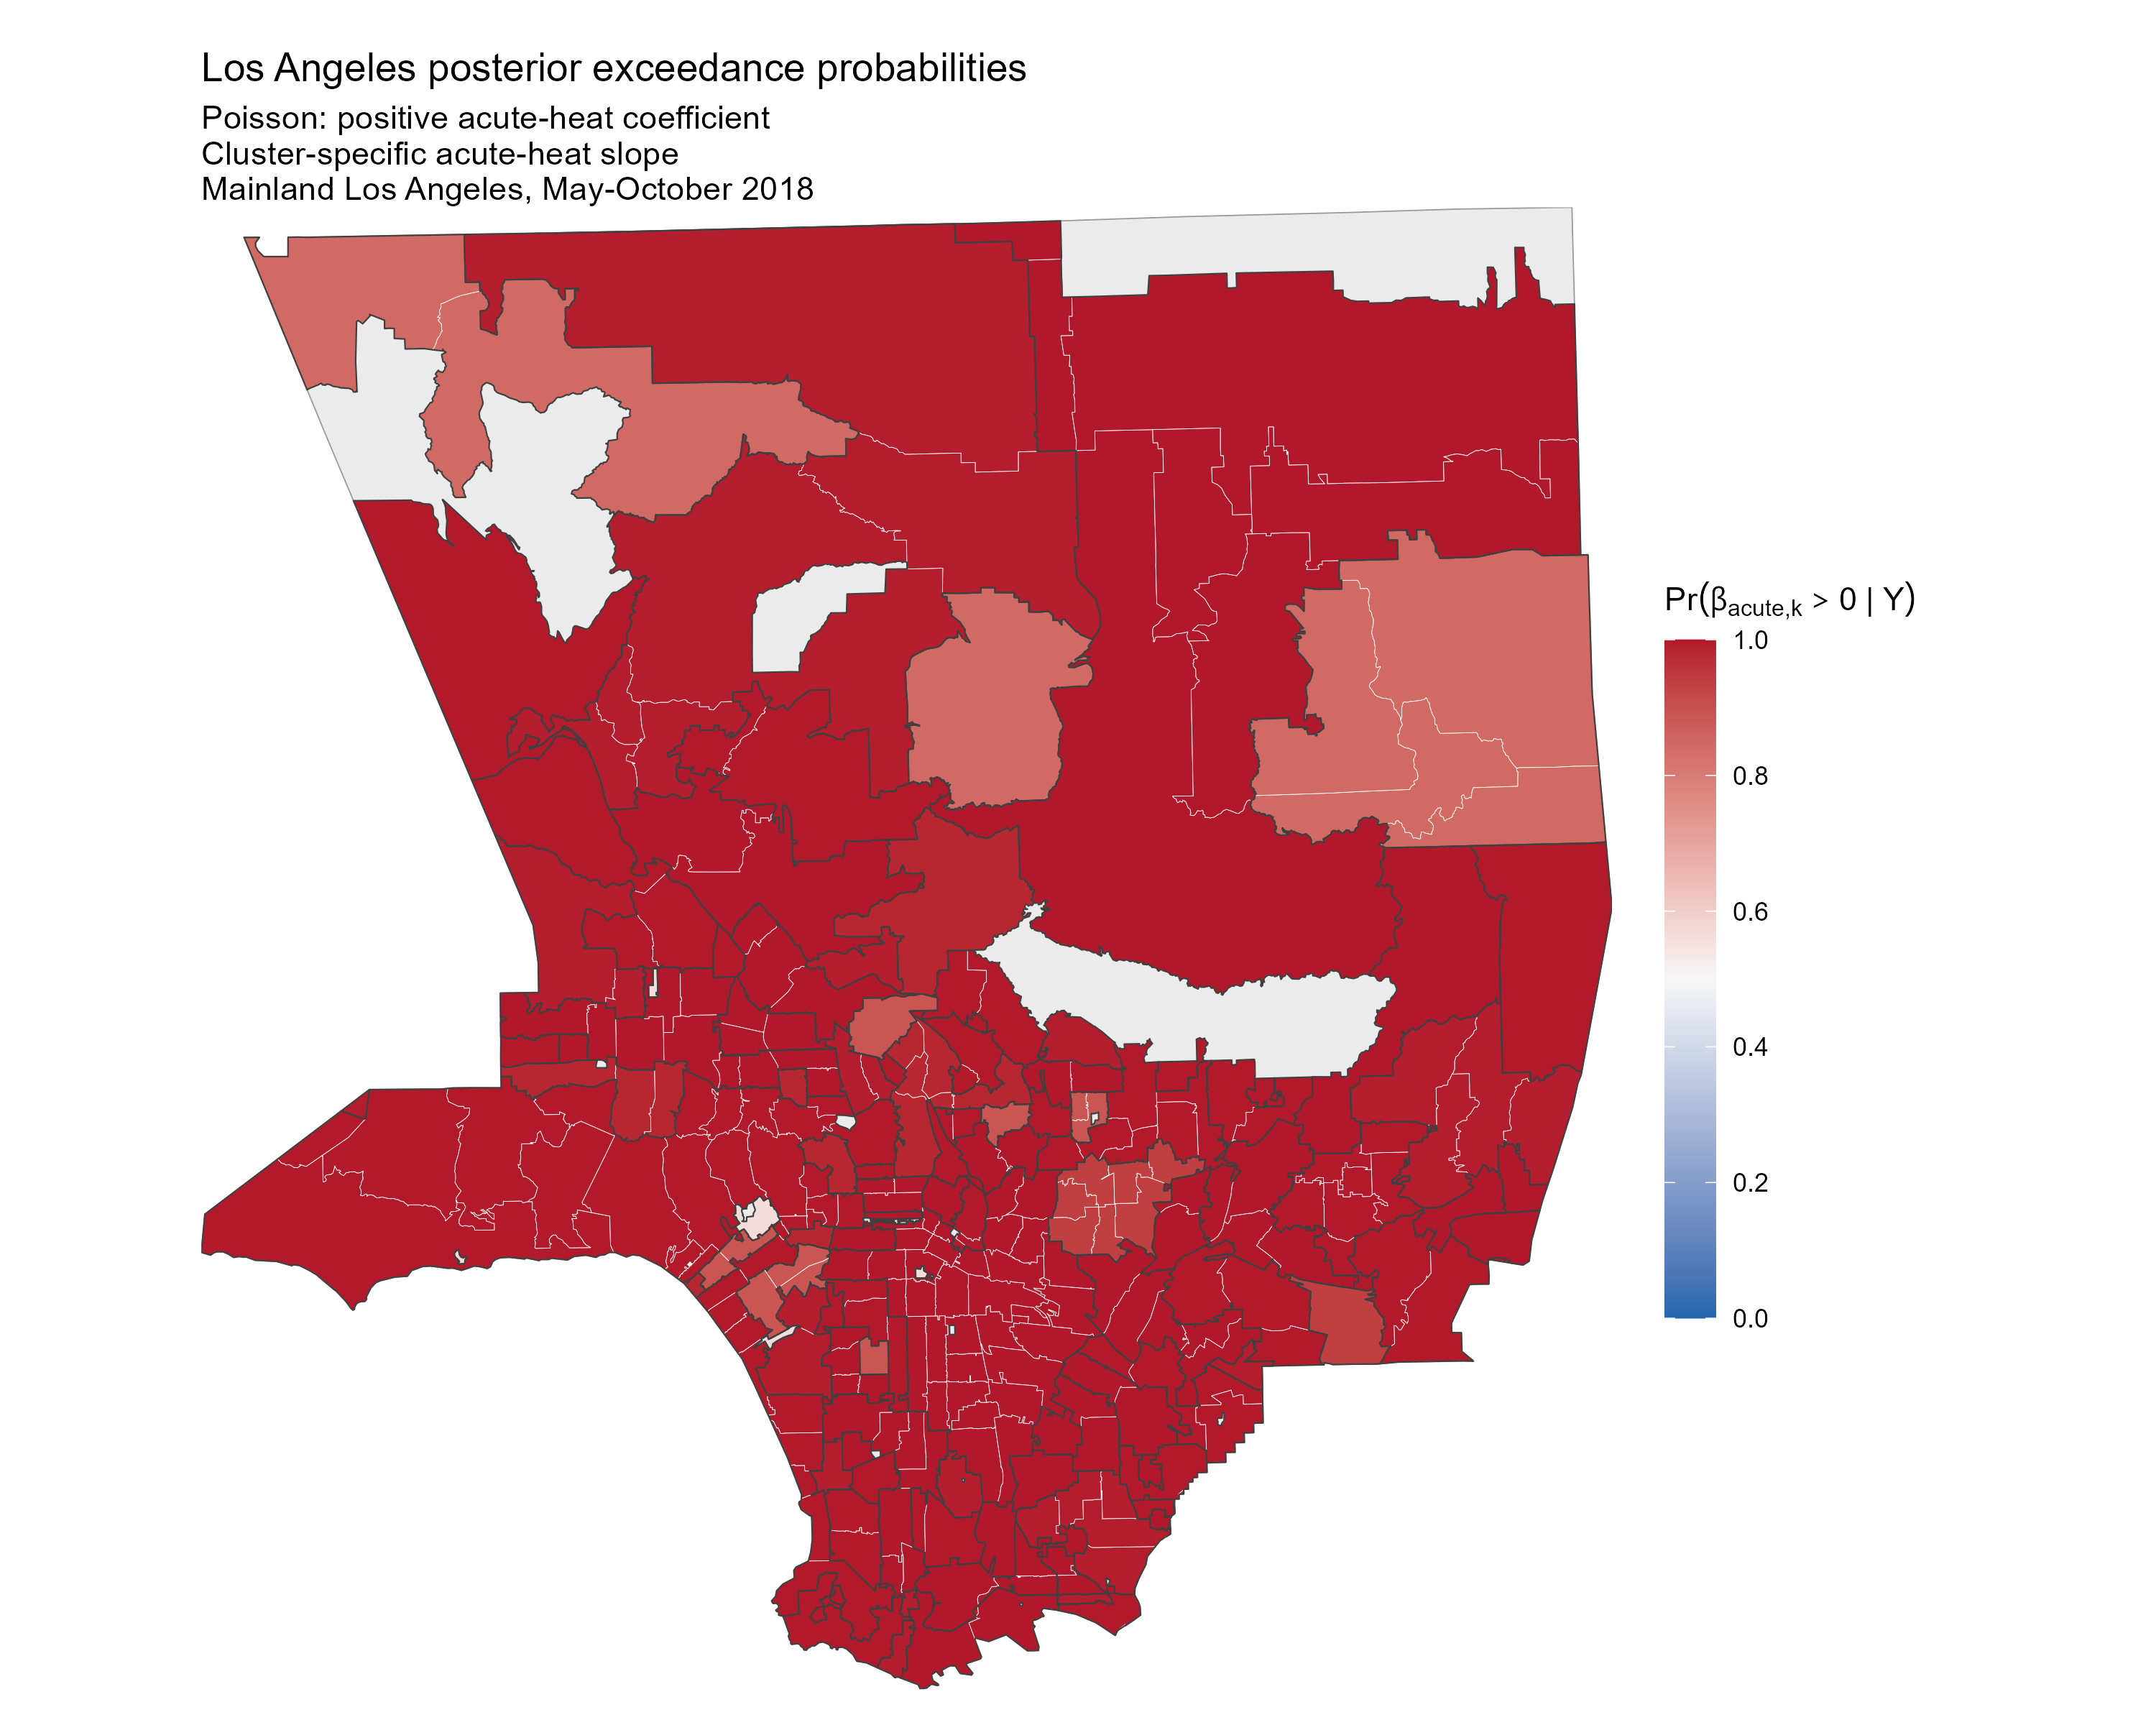
\includegraphics[width=\textwidth,height=0.80\textheight,keepaspectratio]{acute_heat_probability_map_zcta.png}
\caption{Poisson posterior probability that the cluster-specific acute-heat
coefficient exceeds zero, $\Pr(\beta_{\mathrm{acute},k}>0\mid Y)$.
Each assigned ZCTA is colored by its cluster's probability.
Cluster probabilities range from 0.989177 to 0.9999998 on the fixed 0--1 scale.}
\label{fig:probability}
\end{figure}
\clearpage
\begin{figure}[p]
\centering
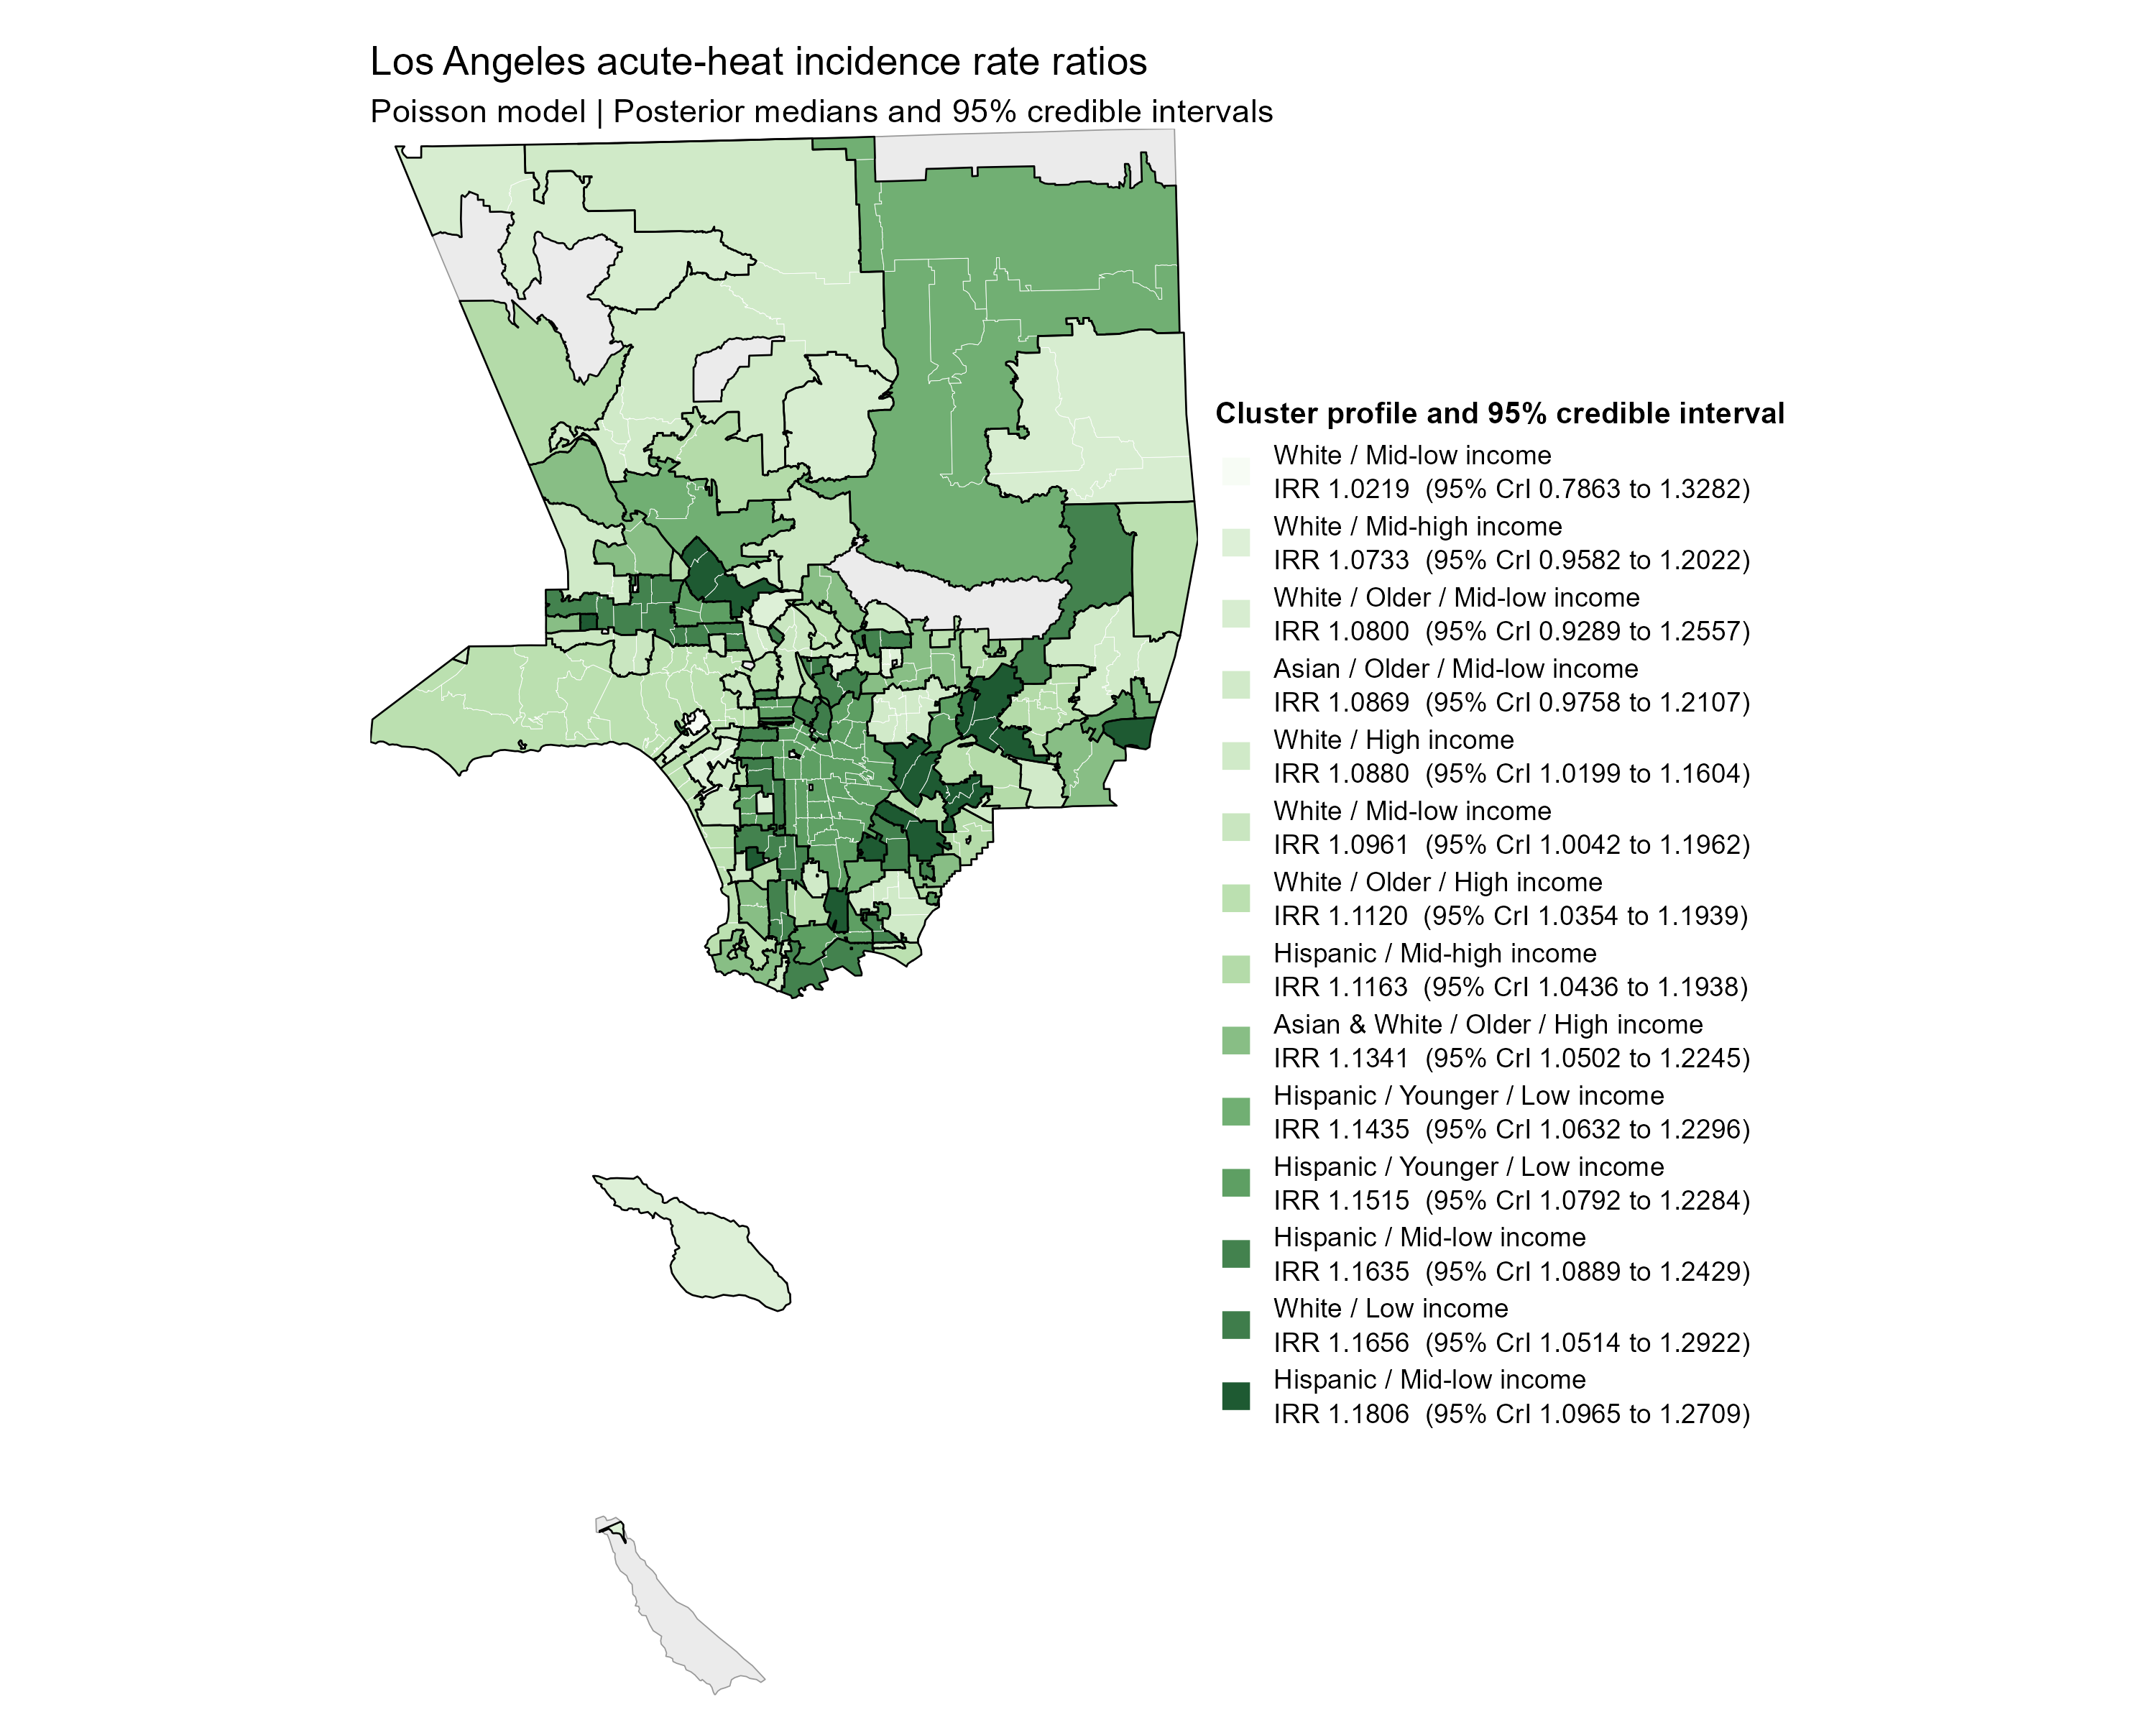
\includegraphics[width=\textwidth,height=0.80\textheight,keepaspectratio]{acute_heat_irr_map.png}
\caption{Poisson acute-heat incidence rate ratios per one pooled SD increase
in acute heat, holding chronic heat and the other model terms fixed.
Colors show posterior medians; the legend gives equal-tail 95\% credible intervals.}
\label{fig:irr}
\end{figure}
\end{document}
